\question
The slope of the curve $y^{3}-x y^{2}=4$ at the point where $y=2$ is
\begin{choices}
  \choice $-2$
  \choice $\dfrac{1}{4}$
  \choice $-\dfrac{1}{2}$
  \CorrectChoice $\dfrac{1}{2}$
  \choice $2$
\end{choices}
\begin{solution}
Substituting $y=2$ yields $x=1$. We find $y^{\prime}$ implicitly.


\[
3 y^{2} y^{\prime}-\left(2 x y y^{\prime}+y^{2}\right)=0 ; \quad\left(3 y^{2}-2 x y\right) y^{\prime}-y^{2}=0 .
\]

Replace $x$ by 1 and $y$ by 2 ; solve for $y^{\prime}$.
\end{solution}

\question
The slope of the curve $y^{2}-x y-3 x=1$ at the point $(0,-1)$ is
\begin{choices}
  \CorrectChoice $-1$
  \choice $-2$
  \choice $+1$
  \choice $2$
  \choice $-3$
\end{choices}
\begin{solution}
(A) $2 y y^{\prime}-\left(x y^{\prime}+y\right)-3=0$. Replace $x$ by 0 and $y$ by -1 ; solve for $y^{\prime}$.
\end{solution}

\question
The equation of the tangent to the curve $y=x \sin x$ at the point $\left(\dfrac{\pi}{2}, \dfrac{\pi}{2}\right)$ is
\begin{choices}
  \choice $y=x-\pi$
  \choice $y=\dfrac{\pi}{2}$
  \choice $y=\pi-x$
  \choice $y=x+\dfrac{\pi}{2}$
  \CorrectChoice $y=x$
\end{choices}
\begin{solution}
(E) Find the slope of the curve at $x=\dfrac{\pi}{2}: y^{\prime}=x \cos x+\sin x$. At $x=\dfrac{\pi}{2}$, $y^{\prime}=\dfrac{\pi}{2} \cdot 0+1$. The equation is $y-\dfrac{\pi}{2}=1\left(x-\dfrac{\pi}{2}\right)$.
\end{solution}


\newpage



\question
The tangent to the curve of $y=x e^{-x}$ is horizontal when $x$ is equal to
\begin{choices}
  \choice $0$
  \CorrectChoice $1$
  \choice $-1$
  \choice $\dfrac{1}{e}$
  \choice none of these
\end{choices}
\begin{solution}
(B) Since $y^{\prime}=e^{-x}(1-x)$ and $e^{-x}>0$ for all $x, y^{\prime}=0$ when $x=1$.
\end{solution}

\question
The minimum value of the slope of the curve $y=x^{5}+x^{3}-2 x$ is
\begin{choices}
  \choice $0$
  \choice $2$
  \choice $6$
  \CorrectChoice $-2$
  \choice none of these
\end{choices}
\begin{solution}
(D) The slope $y^{\prime}=5 x^{4}+3 x^{2}-2$. Let $g=y^{\prime}$. Since $g^{\prime}(x)=20 x^{3}+6 x=2 x\left(10 x^{2}+3\right)$, $g^{\prime}(x)=0$ only if $x=0$. Since $g^{\prime \prime}(x)=60 x^{2}+6, g^{\prime \prime}$ is always positive, assuring that $x=0$ yields the minimum slope. Find $y^{\prime}$ when $x=0$.
\end{solution}

\question
The equation of the tangent to the hyperbola $x^{2}-y^{2}=12$ at the point $(4,2)$ on the curve is
\begin{choices}
  \choice $x-2 y+6=0$
  \choice $y=2 x$
  \CorrectChoice $y=2 x-6$
  \choice $y=\dfrac{x}{2}$
  \choice $x+2 y=6$
\end{choices}
\begin{solution}
(C) Since $2 x-2 y y^{\prime}=0, y^{\prime}=\dfrac{x}{y}$. At $(4,2), y^{\prime}=2$. The equation of the tangent at $(4,2)$ is $y-2=2(x-4)$.
\end{solution}


\newpage



\question
The tangent to the curve $y^{2}-x y+9=0$ is vertical when
\begin{choices}
  \choice $y=0$
  \choice $y= \pm \sqrt{3}$
  \choice $y=\dfrac{1}{2}$
  \CorrectChoice $y= \pm 3$
  \choice none of these
\end{choices}
\begin{solution}
(D) Since $y^{\prime}=\dfrac{y}{2 y-x}$, the tangent is vertical for $x=2 y$. Substitute in the given equation and solve for $y$.
\end{solution}

\question
The best approximation, in cubic inches, to the increase in volume of a sphere when the radius is increased from 3 to 3.1 in . is
\begin{choices}
  \choice $\dfrac{0.04 \pi}{3}$
  \choice $0.04 \pi$
  \choice $1.2 \pi$
  \CorrectChoice $3.6 \pi$
  \choice $36 \pi$
\end{choices}
\begin{solution}
(D) Since $V=\dfrac{4}{3} \pi r^{3}$, therefore, $d V=4 \pi r^{2} d r$. The approximate increase in volume is $d V \approx 4 \pi\left(3^{2}\right)(0.1) \mathrm{in}^{3}$.
\end{solution}

\question
When $x=3$, the equation $2 x^{2}-y^{3}=10$ has the solution $y=2$. When $x=3.04, y \simeq$
\begin{choices}
  \choice $1.6$
  \choice $1.96$
  \CorrectChoice $2.04$
  \choice $2.14$
  \choice $2.4$
\end{choices}
\begin{solution}
(C) Differentiating implicitly yields $4 x-3 y^{2} y^{\prime}=0$. So $y^{\prime}=\dfrac{4 x}{3 y^{2}}$. The linear approximation for the true value of $y$ when $x$ changes from 3 to 3.04 is
\[
y_{\text {at } x=3}+y_{\text {at point }(3,2)}^{\prime} \cdot(3.04-3)
\]
Since it is given that, when $x=3, y=2$, the approximate value of $y$ is
\[
2+\dfrac{4 x}{3 y_{\text {at }(3,2)}^{2}} \cdot(0.04)
\]
or
\[
2+\dfrac{12}{12} \cdot(0.04)=2.04
\]
\end{solution}




\newpage



\question
If the side $e$ of a square is increased by $1 \%$, then the area is increased approximately
\begin{choices}
  \choice $0.02 e$
  \CorrectChoice $0.02 e^{2}$
  \choice $0.01 e^{2}$
  \choice $1 \%$
  \choice $0.01 e$
\end{choices}
\begin{solution}
We want to approximate the change in area of the square when a side of length $e$ increases by $0.01 e$. The answer is


\[
A^{\prime}(e)(0.01 e) \text { or } 2 e(0.01 e)
\]


  \setcounter{enumi}{10}
\end{solution}

\question
The edge of a cube has length 10 in ., with a possible error of $1 \%$. The possible error, in cubic inches, in the volume of the cube is
\begin{choices}
  \choice $3$
  \choice $1$
  \choice $10$
  \CorrectChoice $30$
  \choice none of these
\end{choices}
\begin{solution}
Since $V=e^{3}, V^{\prime}=3 e^{2}$. Therefore at $e=10$, the slope of the tangent line is 300 . The change in volume is approximately $300( \pm 0.1)=30 \mathrm{in} .^{3}$
\end{solution}





\newpage



\question\label{calc04:extrema-quad}
The function $f(x)=x^{4}-4 x^{2}$ has
\begin{choices}
  \choice one relative minimum and two relative maxima
  \choice one relative minimum and one relative maximum
  \choice two relative maxima and no relative minimum
  \choice two relative minima and no relative maximum
  \CorrectChoice two relative minima and one relative maximum
\end{choices}
\begin{solution}
$f^{\prime}(x)=4 x^{3}-8 x=4 x\left(x^{2}-2\right) \cdot f^{\prime}=0$ if $x=0$ or $\pm \sqrt{2}$.
$f^{\prime \prime}(x)=12 x^{2}-8 ; f^{\prime \prime}$ is positive if $x= \pm \sqrt{2}$, negative if $x=0$.
\end{solution}


\question
The number of inflection points of the curve in Question~\ref{calc04:extrema-quad} is
\begin{choices}
  \choice $0$
  \choice $1$
  \CorrectChoice $2$
  \choice $3$
  \choice $4$
\end{choices}
\begin{solution}
Since $f^{\prime \prime}(x)=4\left(3 x^{2}-2\right)$, it equals 0 if $x= \pm \sqrt{\dfrac{2}{3}}$. Since $f^{\prime \prime}$ changes sign as $x$ increases through each of these, both are inflection points.
\end{solution}





\newpage



\question
The maximum value of the function $y=-4 \sqrt{2-x}$ is
\begin{choices}
  \CorrectChoice $0$
  \choice $-4$
  \choice $2$
  \choice $-2$
  \choice none of these
\end{choices}
\begin{solution}
The domain of $y$ is $\{x \mid x \leqq 2\}$. Note that $y$ is negative for each $x$ in the domain except 2 , where $y=0$.
\end{solution}

\question
The total number of local maximum and minimum points of the function whose derivative, for all $x$, is given by $f^{\prime}(x)=x(x-3)^{2}(x+1)^{4}$ is
\begin{choices}
  \choice $0$
  \CorrectChoice $1$
  \choice $2$
  \choice $3$
  \choice none of these
\end{choices}
\begin{solution}
$\quad f^{\prime}(x)$ changes sign only as $x$ passes through zero.
\end{solution}

\question\label{calc04:curve-first}
For which curve shown below are both $f^{\prime}$ and $f^{\prime \prime}$ negative?
\\
\begin{oneparchoices}
\choice
\begin{minipage}[t]{0.28\linewidth}
  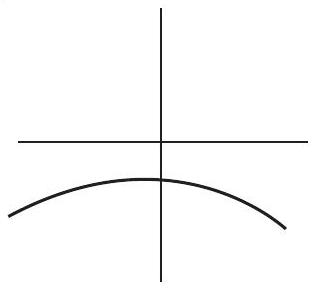
\includegraphics[width=\linewidth]{calculus/images/7914d111-1a3f-478e-8520-371cc22a7467-02_291_319_1660_417.jpg}
\end{minipage}
\choice
\begin{minipage}[t]{0.28\linewidth}
  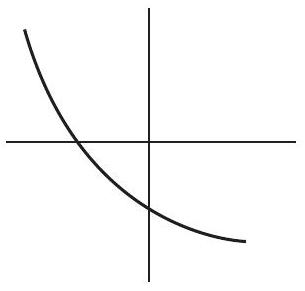
\includegraphics[width=\linewidth]{calculus/images/7914d111-1a3f-478e-8520-371cc22a7467-02_291_305_1660_881.jpg}
\end{minipage}
\choice
\begin{minipage}[t]{0.28\linewidth}
  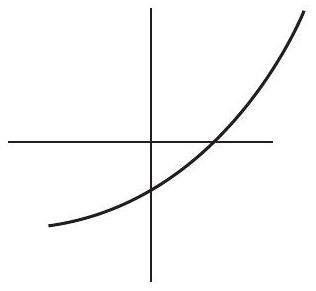
\includegraphics[width=\linewidth]{calculus/images/7914d111-1a3f-478e-8520-371cc22a7467-02_291_316_1660_1331.jpg}
\end{minipage}
\par\vspace{10pt}\noindent
\choice
\begin{minipage}[t]{0.28\linewidth}
  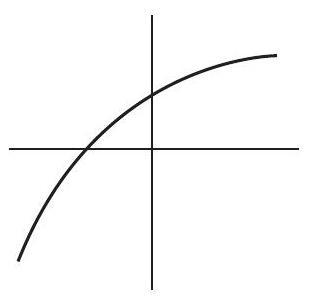
\includegraphics[width=\linewidth]{calculus/images/7914d111-1a3f-478e-8520-371cc22a7467-02_300_312_2036_426.jpg}
\end{minipage}
\CorrectChoice
\begin{minipage}[t]{0.28\linewidth}
  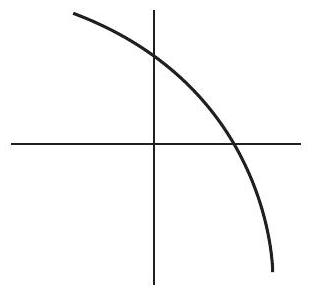
\includegraphics[width=\linewidth]{calculus/images/7914d111-1a3f-478e-8520-371cc22a7467-02_293_314_2041_876.jpg}
\end{minipage}
\end{oneparchoices}
\begin{solution}
The graph must be decreasing and concave downward.
\end{solution}


\newpage


\question\label{calc04:curve-second}
For which curve shown in Question~\ref{calc04:curve-first} is $f^{\prime \prime}$ positive but $f^{\prime}$ negative?
\\
\begin{oneparchoices}
\CorrectChoice
\begin{minipage}[t]{0.28\linewidth}
  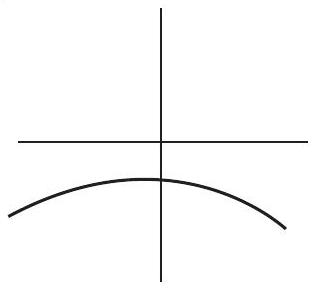
\includegraphics[width=\linewidth]{calculus/images/7914d111-1a3f-478e-8520-371cc22a7467-02_291_319_1660_417.jpg}
\end{minipage}
\choice
\begin{minipage}[t]{0.28\linewidth}
  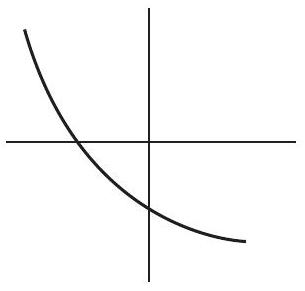
\includegraphics[width=\linewidth]{calculus/images/7914d111-1a3f-478e-8520-371cc22a7467-02_291_305_1660_881.jpg}
\end{minipage}
\choice
\begin{minipage}[t]{0.28\linewidth}
  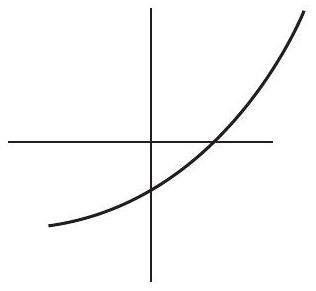
\includegraphics[width=\linewidth]{calculus/images/7914d111-1a3f-478e-8520-371cc22a7467-02_291_316_1660_1331.jpg}
\end{minipage}
\par\vspace{10pt}\noindent
\choice
\begin{minipage}[t]{0.28\linewidth}
  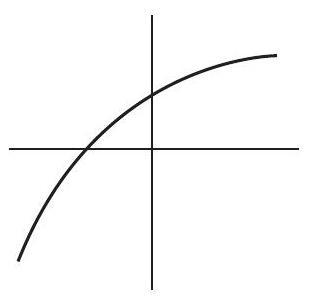
\includegraphics[width=\linewidth]{calculus/images/7914d111-1a3f-478e-8520-371cc22a7467-02_300_312_2036_426.jpg}
\end{minipage}
\choice
\begin{minipage}[t]{0.28\linewidth}
  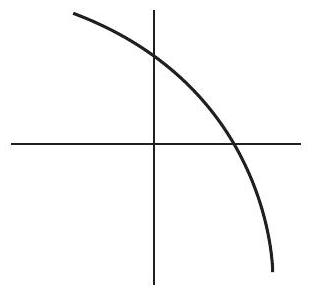
\includegraphics[width=\linewidth]{calculus/images/7914d111-1a3f-478e-8520-371cc22a7467-02_293_314_2041_876.jpg}
\end{minipage}
\end{oneparchoices}
\begin{solution}
The graph must be concave upward but decreasing.
\end{solution}




\newpage




\begin{EnvFullwidth}
\textit{In Questions~\ref{calc04:particle1-first}--\ref{calc04:particle1-last}, the position of a particle moving along a straight line is given by $s=t^{3}-6 t^{2}+12 t-8$.}
\end{EnvFullwidth}

\question\label{calc04:particle1-first}
The distance $s$ is increasing for
\begin{choices}
  \choice $t<2$
  \CorrectChoice all $t$ except $t=2$
  \choice $1<t<3$
  \choice $t<1$ or $t>3$
  \choice $t>2$
\end{choices}
\begin{solution}
The distance is increasing when $v$ is positive. Since $v=\dfrac{d s}{d t}=3(t-2)^{2}$, $v>0$ for all $t \neq 2$.
\end{solution}

\question
The minimum value of the speed is
\begin{choices}
  \choice $1$
  \choice $2$
  \choice $3$
  \CorrectChoice $0$
  \choice none of these
\end{choices}
\begin{solution}
The speed $=|v|$. From Question~\ref{calc04:particle1-first}, $|v|=v$. The least value of $v$ is 0 .
\end{solution}

\question
The acceleration is positive
\begin{choices}
  \CorrectChoice when $t>2$
  \choice for all $t, t \neq 2$
  \choice when $t<2$
  \choice for $1<t<3$
  \choice for $1<t<2$
\end{choices}
\begin{solution}
The acceleration $a=\dfrac{d v}{d t}$. From Question~\ref{calc04:particle1-first}, $a=6(t-2)$.
\end{solution}

\question\label{calc04:particle1-last}
The speed of the particle is decreasing for
\begin{choices}
  \choice $t>2$
  \choice $t<3$
  \choice all $t$
  \choice $t<1$ or $t>2$
  \CorrectChoice none of these
\end{choices}
\begin{solution}
The speed is decreasing when $v$ and $a$ have opposite signs. The answer is $t<2$, since for all such $t$ the velocity is positive while the acceleration is negative. For $t>2$, both $v$ and $a$ are positive.
\end{solution}





\newpage




\begin{EnvFullwidth}
\textit{In Questions~\ref{calc04:particle2-first}--\ref{calc04:particle2-last}, a particle moves along a horizontal line and its position at time $t$ is $s=t^{4}-6 t^{3}+12 t^{2}+3$.}
\end{EnvFullwidth}

\question\label{calc04:particle2-first}
The particle is at rest when $t$ is equal to
\begin{choices}
  \choice $1$ or $2$
  \CorrectChoice $0$
  \choice $\dfrac{9}{4}$
  \choice $0$,$2$ , or $3$
  \choice none of these
\end{choices}
\begin{solution}
The particle is at rest when $v=0 ; v=2 t\left(2 t^{2}-9 t+12\right)=0$ only if $t=0$. Note that the discriminant of the quadratic factor $\left(b^{2}-4 a c\right)$ is negative.
\end{solution}

\question
The velocity, $v$, is increasing when
\begin{choices}
  \choice $t>1$
  \choice $1<t<2$
  \choice $t<2$
  \CorrectChoice $t<1$ or $t>2$
  \choice $t>0$
\end{choices}
\begin{solution}
Since $a=12(t-1)(t-2)$, we check the signs of $a$ in the intervals $t<1$, $1<t<2$, and $t>2$. We choose those where $a>0$.
\end{solution}

\question\label{calc04:particle2-last}
The speed of the particle is increasing for
\begin{choices}
  \CorrectChoice $0<t<1$ or $t>2$
  \choice $1<t<2$
  \choice $t<2$
  \choice $t<0$ or $t>2$
  \choice $t<0$
\end{choices}
\begin{solution}
From Questions~\ref{calc04:particle2-first} and the preceding question we see that $v>0$ if $t>0$ and that $a>0$ if $t<1$ or $t>2$. So both $v$ and $a$ are positive if $0<t<1$ or $t>2$. There are no values of $t$ for which both $v$ and $a$ are negative.
\end{solution}





\newpage




\question
The displacement from the origin of a particle moving on a line is given by $s= t^{4}-4 t^{3}$. The maximum displacement during the time interval $-2 \leqq t \leqq 4$ is
\begin{choices}
  \choice $27$
  \choice $3$
  \choice $12 \sqrt{3}+3$
  \CorrectChoice $48$
  \choice none of these
\end{choices}
\begin{solution}
See the figure, which shows the motion of the particle during the time interval $-2 \leqslant t \leqslant 4$. The particle is at rest when $t=0$ or 3 , but reverses direction only at 3 . The endpoints need to be checked here, of course. Indeed, the maximum displacement occurs at one of those, namely, when $t=-2$.\\
\begin{center}
  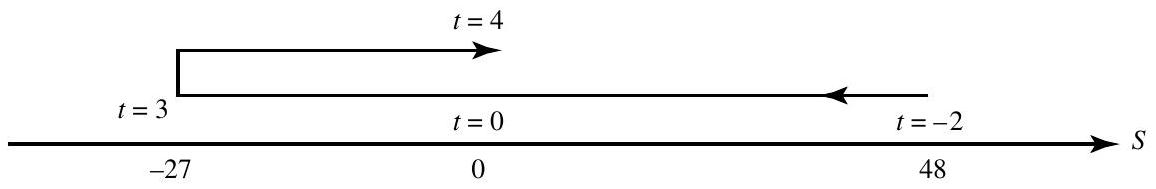
\includegraphics[width=0.7\linewidth]{calculus/images/7914d111-1a3f-478e-8520-371cc22a7467-17_189_1156_681_881.jpg}
\end{center}
\end{solution}

\question
If a particle moves along a line according to the law $s=t^{5}+5 t^{4}$, then the number of times it reverses direction is
\begin{choices}
  \choice $0$
  \choice $1$
  \CorrectChoice $2$
  \choice $3$
  \choice $4$
\end{choices}
\begin{solution}
Since $v=5 t^{3}(t+4), v=0$ when $t=-4$ or 0 . Note that $v$ does change sign at each of these times.
\end{solution}





\newpage




\begin{EnvFullwidth}
\textit{In Questions~\ref{calc04:vector-first}--\ref{calc04:vector-last}, $\mathbf{R}=3 \cos \dfrac{\pi}{3} t \mathbf{i}+2 \sin \dfrac{\pi}{3} t \mathbf{j}$ is the (position) vector $x \mathbf{i}+y \mathbf{j}$ from the origin to a moving point $P(x, y)$ at time $t$.}
\end{EnvFullwidth}

\question\label{calc04:vector-first}
A single equation in $x$ and $y$ for the path of the point is
\begin{choices}
  \choice $x^{2}+y^{2}=13$
  \choice $9 x^{2}+4 y^{2}=36$
  \choice $2 x^{2}+3 y^{2}=13$
  \choice $4 x^{2}+9 y^{2}=1$
  \CorrectChoice $4 x^{2}+9 y^{2}=36$
\end{choices}
\begin{solution}
Since $x=3 \cos \dfrac{\pi}{3} t$ and $y=2 \sin \dfrac{\pi}{3} t$, we note that $\left(\dfrac{x}{3}\right)^{2}+\left(\dfrac{y}{2}\right)^{2}=1$.
\end{solution}

\question
When $t=3$, the speed of the particle is
\begin{choices}
  \CorrectChoice $\dfrac{2 \pi}{3}$
  \choice $2$
  \choice $3$
  \choice $\pi$
  \choice $\dfrac{\sqrt{13}}{3} \pi$
\end{choices}
\begin{solution}
Note that $\mathbf{v}=-\pi \sin \dfrac{\pi}{3} t \mathbf{i}+\dfrac{2 \pi}{3} \cos \dfrac{\pi}{3} t \mathbf{j}$. At $t=3$,


\[
|\mathbf{v}|=\sqrt{(-\pi \cdot 0)^{2}+\left(\dfrac{2 \pi}{3} \cdot-1\right)^{2}}
\]


  \setcounter{enumi}{28}
\end{solution}

\question
The magnitude of the acceleration when $t=3$ is
\begin{choices}
  \choice $2$
  \CorrectChoice $\dfrac{\pi^{2}}{3}$
  \choice $3$
  \choice $\dfrac{2 \pi^{2}}{9}$
  \choice $\pi$
\end{choices}
\begin{solution}
$\quad \mathbf{a}=-\dfrac{\pi^{2}}{3} \cos \dfrac{\pi}{3} t \mathbf{i}-\dfrac{2 \pi^{2}}{9} \sin \dfrac{\pi}{3} t \mathbf{j}$. At $t=3$,
\[
|\mathbf{a}|=\sqrt{\left(\dfrac{-\pi^{2}}{3} \cdot-1\right)^{2}+\left(\dfrac{-2 \pi^{2}}{9} \cdot 0\right)^{2}}
\]
\end{solution}





\newpage




\question\label{calc04:vector-last}
At the point where $t=\dfrac{1}{2}$, the slope of the curve along which the particle moves is
\begin{choices}
  \choice $-\dfrac{2 \sqrt{3}}{9}$
  \choice $-\dfrac{\sqrt{3}}{2}$
  \choice $\dfrac{2}{\sqrt{3}}$
  \CorrectChoice $-\dfrac{2 \sqrt{3}}{3}$
  \choice none of these
\end{choices}
\begin{solution}
The slope of the curve is the slope of $\mathbf{v}$, namely, $\dfrac{\dfrac{d y}{d t}}{\dfrac{d x}{d t}}$. At $t=\dfrac{1}{2}$, the slope\\
is equal to


\[
\dfrac{\dfrac{2 \pi}{3} \cdot \cos \dfrac{\pi}{6}}{-\pi \cdot \sin \dfrac{\pi}{6}}=-\dfrac{2}{3} \cot \dfrac{\pi}{6} .
\]


  \setcounter{enumi}{30}
\end{solution}

\question
A balloon is being filled with helium at the rate of $4 \mathrm{ft}^{3} / \mathrm{min}$. The rate, in square feet per minute, at which the surface area is increasing when the volume is $\dfrac{32 \pi}{3} \mathrm{ft}^{3}$ is
\begin{choices}
  \choice $4 \pi$
  \choice $2$
  \CorrectChoice $4$
  \choice $1$
  \choice $2 \pi$
\end{choices}
\begin{solution}
Since $V=\dfrac{4}{3} \pi r^{3}, \dfrac{d V}{d t}=4 \pi r^{2} \dfrac{d r}{d t}$. Since $\dfrac{d V}{d t}=4, \dfrac{d r}{d t}=\dfrac{1}{\pi r^{2}}$. When $V=\dfrac{32 \pi}{3}$, $r=2$ and $\dfrac{d r}{d t}=\dfrac{1}{4 \pi}$.
\[
S=4 \pi r^{2} ; \quad \dfrac{d S}{d t}=8 \pi r \dfrac{d r}{d t}
\]
when $r=2, \dfrac{d S}{d t}=8 \pi(2)\left(\dfrac{1}{4 \pi}\right)=4$.
\end{solution}





\newpage




\question
A circular conical reservoir, vertex down, has depth 20 ft and radius of the top 10 ft . Water is leaking out so that the surface is falling at the rate of $\dfrac{1}{2} \mathrm{ft} / \mathrm{hr}$. The rate, in cubic feet per hour, at which the water is leaving the reservoir when the water is 8 ft deep is
\begin{choices}
  \choice $4 \pi$
  \CorrectChoice $8 \pi$
  \choice $16 \pi$
  \choice $\dfrac{1}{4 \pi}$
  \choice $\dfrac{1}{8 \pi}$
\end{choices}
\begin{solution}
(B) See Figure N4-22 on page 189. Replace the printed measurements of the radius and height by 10 and 20 , respectively. We are given here that $r=\dfrac{h}{2}$ and that $\dfrac{d h}{d t}=-\dfrac{1}{2}$. Since $V=\dfrac{1}{3} \pi r^{2} h$, we have $V=\dfrac{\pi}{3} \dfrac{h^{3}}{4}$, so
\[
\dfrac{d V}{d t}=\dfrac{\pi h^{2}}{4} \dfrac{d h}{d t}=\dfrac{-\pi h^{2}}{8}
\]
Replace $h$ by 8.
\end{solution}

\question
A local minimum value of the function $y=\dfrac{e^{x}}{x}$ is
\begin{choices}
  \choice $\dfrac{1}{e}$
  \choice $1$
  \choice $-1$
  \CorrectChoice $e$
  \choice $0$
\end{choices}
\begin{solution}
(D) $y^{\prime}=\dfrac{e^{x}(x-1)}{x^{2}}(x \neq 0)$. Since $y^{\prime}=0$ if $x=1$ and changes from negative to positive as $x$ increases through $1, x=1$ yields a minimum. Evaluate $y$ at $x=1$.
\end{solution}





\newpage




\question
The area of the largest rectangle that can be drawn with one side along the $x$-axis and two vertices on the curve of $y=e^{-x^{2}}$ is
\begin{choices}
  \CorrectChoice $\sqrt{\dfrac{2}{e}}$
  \choice $\sqrt{2 e}$
  \choice $\dfrac{2}{e}$
  \choice $\dfrac{1}{\sqrt{2 e}}$
  \choice $\dfrac{2}{e^{2}}$
\end{choices}
\begin{solution}
(A) The domain of $y$ is $-\infty<x<\infty$. The graph of $y$, which is nonnegative, is symmetric to the $y$-axis. The inscribed rectangle has area $A=2 x e^{-x^{2}}$. Thus $A^{\prime}=\dfrac{2\left(1-2 x^{2}\right)}{e^{x^{2}}}$, which is 0 when the positive value of $x$ is $\dfrac{\sqrt{2}}{2}$. This value of $x$ yields maximum area. Evaluate $A$.
\end{solution}

\question
A line is drawn through the point $(1,2)$ forming a right triangle with the positive $x$- and $y$-axes.
The slope of the line forming the triangle of least area is
\begin{choices}
  \choice $-1$
  \CorrectChoice $-2$
  \choice $-4$
  \choice $-\dfrac{1}{2}$
  \choice $-3$
\end{choices}
\begin{solution}
(B) See the figure. If we let $m$ be the slope of the line, then its equation is $y-2= m(x-1)$ with intercepts as indicated in the figure.\\
\begin{center}
  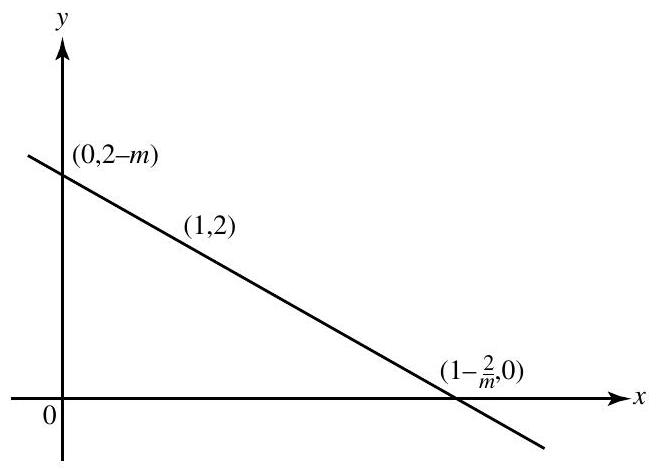
\includegraphics[width=0.40\linewidth]{calculus/images/7914d111-1a3f-478e-8520-371cc22a7467-18_469_657_1308_663.jpg}
\end{center}
The area $A$ of the triangle is given by

\[
A=\dfrac{1}{2}(2-m)\left(1-\dfrac{2}{m}\right)=\dfrac{1}{2}\left(4-\dfrac{4}{m}-m\right) .
\]

Then $\dfrac{d A}{d m}=\dfrac{1}{2}\left(\dfrac{4}{m^{2}}-1\right)$ and equals 0 when $m= \pm 2 ; m$ must be negative.
\end{solution}





\newpage




\question
The point(s) on the curve $x^{2}-y^{2}=4$ closest to the point ( 6,0 ) is (are)
\begin{choices}
  \choice $(2,0)$
  \choice $(\sqrt{5}, \pm 1)$
  \CorrectChoice $(3, \pm \sqrt{5})$
  \choice $(\sqrt{13}, \pm \sqrt{3})$
  \choice none of these
\end{choices}
\begin{solution}
(C) Let $q=(x-6)^{2}+y^{2}$ be the quantity to be minimized. Then

\[
q=(x-6)^{2}+\left(x^{2}-4\right)
\]

$q^{\prime}=0$ when $x=3$. Note that it suffices to minimize the square of the distance.
\end{solution}

\question
The sum of the squares of two positive numbers is 200 ; their minimum product is
\begin{choices}
  \choice $100$
  \choice $25 \sqrt{7}$
  \choice $28$
  \choice $24 \sqrt{14}$
  \CorrectChoice none of these
\end{choices}
\begin{solution}
(E) Minimize, if possible, $x y$, where $x^{2}+y^{2}=200(x, y>0)$. The derivative of the product is $\dfrac{2\left(100-x^{2}\right)}{\sqrt{200-x^{2}}}$, which equals 0 for $x=10$. But the signs of the derivative as $x$ increases through 10 show that 10 yields a maximum product. No minimum exists.
\end{solution}

\question
The first-quadrant point on the curve $y^{2} x=18$ that is closest to the point $(2,0)$ is
\begin{choices}
  \choice $(2,3)$
  \choice $(6, \sqrt{3})$
  \CorrectChoice $(3, \sqrt{6})$
  \choice $(1,3 \sqrt{2})$
  \choice none of these
\end{choices}
\begin{solution}
(C) Minimize $q=(x-2)^{2}+\dfrac{18}{x}$. Since
\[
q^{\prime}=2(x-2)-\dfrac{18}{x^{2}}=\dfrac{2\left(x^{3}-2 x^{2}-9\right)}{x^{2}},
\]
$q^{\prime}=0$ if $x=3$. The signs of $q^{\prime}$ about $x=3$ assure a minimum.
\end{solution}





\newpage




\question
If $h$ is a small negative number, then the best approximation for $\sqrt[3]{27+h}$ is
\begin{choices}
  \CorrectChoice $3+\dfrac{h}{27}$
  \choice $3-\dfrac{h}{27}$
  \choice $\dfrac{h}{27}$
  \choice $-\dfrac{h}{27}$
  \choice $3-\dfrac{h}{9}$
\end{choices}
\begin{solution}
(A) The best approximation for $\sqrt[3]{27+h}$ when $h$ is small is the local linear (or tangent line) approximation. If we let $f(h)=\sqrt[3]{27+h}$, then $f^{\prime}(h)=\dfrac{1}{3(27+h)^{2 / 3}}$ and $f^{\prime}(0)=\dfrac{1}{3 \cdot 9}$. The approximation for $f(h)$ is $f(0)+f^{\prime}(0) \cdot h$, which equals $3+\dfrac{1}{27} h$.
\end{solution}

\question
If $f(x)=x e^{-x}$, then at $x=0$
\begin{choices}
  \CorrectChoice $f$ is increasing
  \choice $f$ is decreasing
  \choice $f$ has a relative maximum
  \choice $f$ has a relative minimum
  \choice $f^{\prime}$ does not exist
\end{choices}
\begin{solution}
(A) Since $f^{\prime}(x)=e^{-x}(1-x), f^{\prime}(0)>0$.
\end{solution}





\newpage




\question
A function $f$ has a derivative for each $x$ such that $|x|<2$ and has a local minimum at $(2,-5)$. Which statement below must be true?
\begin{choices}
  \choice $f^{\prime}(2)=0$.
  \choice $f^{\prime}$ exists at $x=2$.
  \choice The graph is concave up at $x=2$.
  \choice $f^{\prime}(x)<0$ if $x<2, f^{\prime}(x)>0$ if $x>2$.
  \CorrectChoice None of the preceding is necessarily true.
\end{choices}
\begin{solution}
(E) The graph shown serves as a counterexample for A-D.\\
\begin{center}
  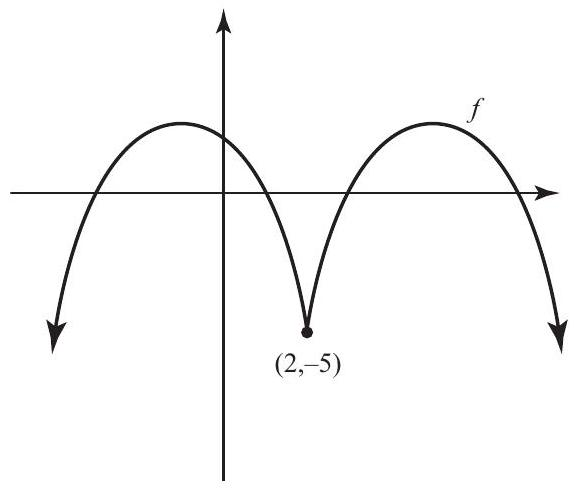
\includegraphics[width=0.40\linewidth]{calculus/images/7914d111-1a3f-478e-8520-371cc22a7467-19_488_578_1143_1062.jpg}
\end{center}
\end{solution}

\question
The height of a rectangular box is 10 in . Its length increases at the rate of $2 \mathrm{in} . / \mathrm{sec}$; its width decreases at the rate of $4 \mathrm{in} . / \mathrm{sec}$. When the length is 8 in . and the width is 6 in ., the rate, in cubic inches per second, at which the volume of the box is changing is
\begin{choices}
  \choice $200$
  \choice $80$
  \choice $-80$
  \CorrectChoice $-200$
  \choice $-20$
\end{choices}
\begin{solution}
(D) Since $V=10 \ell w, V^{\prime}=10\left(\ell \dfrac{d w}{d t}+w \dfrac{d \ell}{d t}\right)=10(8 \cdot-4+6 \cdot 2)$.
\end{solution}





\newpage




\question
The tangent to the curve $x^{3}+x^{2} y+4 y=1$ at the point $(3,-2)$ has slope
\begin{choices}
  \choice $-3$
  \choice $-\dfrac{23}{9}$
  \choice $-\dfrac{27}{13}$
  \choice $-\dfrac{11}{9}$
  \CorrectChoice $-\dfrac{15}{13}$
\end{choices}
\begin{solution}
(E) We differentiate implicitly: $3 x^{2}+x^{2} y^{\prime}+2 x y+4 y^{\prime}=0$. Then $y^{\prime}=-\dfrac{3 x^{2}+2 x y}{x^{2}+4}$. At $(3,-2), y^{\prime}=-\dfrac{27-12}{9+4}=-\dfrac{15}{13}$.
\end{solution}

\question
If $f(x)=a x^{4}+b x^{2}$ and $a b>0$, then
\begin{choices}
  \choice the curve has no horizontal tangents
  \choice the curve is concave up for all $x$
  \choice the curve is concave down for all $x$
  \CorrectChoice the curve has no inflection point
  \choice none of the preceding is necessarily true
\end{choices}
\begin{solution}
(D) Since $a b>0, a$ and $b$ have the same sign; therefore $f^{\prime \prime}(x)=12 a x^{2}+2 b$ never equals 0 . The curve has one horizontal tangent at $x=0$.
\end{solution}

\question
A function $f$ is continuous and differentiable on the interval $[0,4]$, where $f^{\prime}$ is positive but $f^{\prime \prime}$ is negative. Which table could represent points on $f$ ?
\begin{choices}
  \choice \begin{center}
\begin{tabular}{l|c|c|c|c|c}
$x$ & $0$ & $1$ & $2$ & $3$ & $4$ \\
\hline
$y$ & $10$ & $12$ & $14$ & $16$ & $18$ \\
\end{tabular}
\end{center}
  \choice \begin{center}
\begin{tabular}{l|c|c|c|c|c}
$x$ & $0$ & $1$ & $2$ & $3$ & $4$ \\
\hline
$y$ & $10$ & $12$ & $15$ & $19$ & $24$ \\
\end{tabular}
\end{center}
  \CorrectChoice \begin{center}
\begin{tabular}{c|c|c|c|c|c}
$x$ & $0$ & $1$ & $2$ & $3$ & $4$ \\
\hline
$y$ & $10$ & $18$ & $24$ & $28$ & $30$ \\
\end{tabular}
\end{center}
  \choice \begin{center}
\begin{tabular}{l|c|c|c|c|c}
$x$ & $0$ & $1$ & $2$ & $3$ & $4$ \\
\hline
$y$ & $30$ & $28$ & $24$ & $18$ & $10$ \\
\end{tabular}
\end{center}
  \choice \begin{center}
\begin{tabular}{l|c|c|c|c|c}
$x$ & $0$ & $1$ & $2$ & $3$ & $4$ \\
\hline
$y$ & $24$ & $19$ & $15$ & $12$ & $10$ \\
\end{tabular}
\end{center}
\end{choices}
\begin{solution}
(C) Since the first derivative is positive, the function must be increasing. However, the negative second derivative indicates that the rate of increase is slowing down, as seen in table C .
\end{solution}





\newpage




\question
The equation of the tangent to the curve with parametric equations $x=2 t+1, y=3-t^{3}$ at the point where $t=1$ is
\begin{choices}
  \choice $2 x+3 y=12$
  \CorrectChoice $3 x+2 y=13$
  \choice $6 x+y=20$
  \choice $3 x-2 y=5$
  \choice none of these
\end{choices}
\begin{solution}
(B) Since $\dfrac{d y}{d x}=-\dfrac{3 t^{2}}{2}$, therefore, at $t=1, \dfrac{d y}{d x}=-\dfrac{3}{2}$. Also, $x=3$ and $y=2$.
\end{solution}

\question
Approximately how much less than 4 is $\sqrt[3]{63}$ ?
\begin{choices}
  \CorrectChoice $\dfrac{1}{48}$
  \choice $\dfrac{1}{16}$
  \choice $\dfrac{1}{3}$
  \choice $\dfrac{2}{3}$
  \choice $1$
\end{choices}
\begin{solution}
(A) Let $f(x)=x^{1 / 3}$, and find the slope of the tangent line at ( 64,4 ). Since $f^{\prime}(x)= \dfrac{1}{3} x^{-2 / 3}, f^{\prime}(64)=\dfrac{1}{48}$. If we move one unit to the left of 64 , the tangent line will drop approximately $\dfrac{1}{48}$ unit.
\end{solution}

\question
The best linear approximation for $f(x)=\tan x$ near $x=\dfrac{\pi}{4}$ is
\begin{choices}
  \choice $1+\dfrac{1}{2}\left(x-\dfrac{\pi}{4}\right)$
  \choice $1+\left(x-\dfrac{\pi}{4}\right)$
  \choice $1+\sqrt{2}\left(x-\dfrac{\pi}{4}\right)$
  \CorrectChoice $1+2\left(x-\dfrac{\pi}{4}\right)$
  \choice $2+2\left(x-\dfrac{\pi}{4}\right)$
\end{choices}
\begin{solution}
(D) $\quad \tan x \simeq \tan \left(\dfrac{\pi}{4}\right)+\sec ^{2}\left(\dfrac{\pi}{4}\right)\left(x-\dfrac{\pi}{4}\right)=1+2\left(x-\dfrac{\pi}{4}\right)$
\end{solution}





\newpage




\question
When $h$ is near zero, $e^{k h}$, using the tangent-line approximation, is approximately
\begin{choices}
  \choice $k$
  \choice $k h$
  \choice $1$
  \choice $1+k$
  \CorrectChoice $1+k h$
\end{choices}
\begin{solution}
(E) $e^{k h} \simeq e^{k \cdot 0}+k e^{k \cdot 0}(h-0)=1+k h$
\end{solution}

\question
If $f(x)=c x^{2}+d x+e$ for the function shown in the graph, then
\begin{center}
  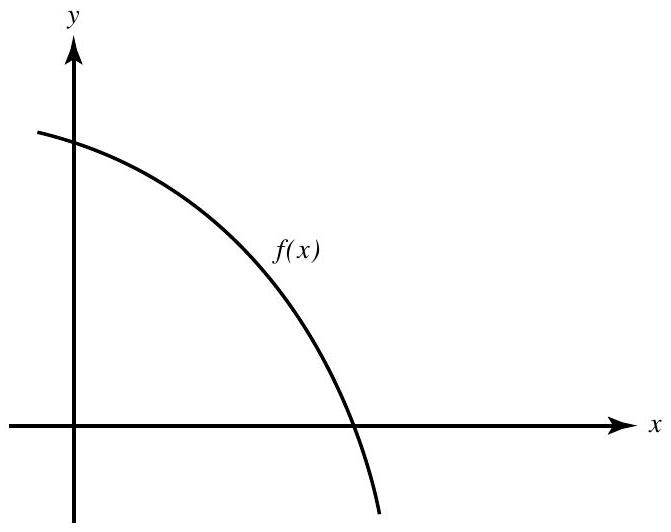
\includegraphics[width=0.60\linewidth]{calculus/images/7914d111-1a3f-478e-8520-371cc22a7467-07_532_671_408_1020.jpg}
\end{center}
\begin{choices}
  \choice $c, d$, and $e$ are all positive
  \choice $c>0, d<0, e<0$
  \choice $c>0, d<0, e>0$
  \choice $c<0, d>0, e>0$
  \CorrectChoice $c<0, d<0, e>0$
\end{choices}
\begin{solution}
(E) Since the curve has a positive $y$-intercept, $e>0$. Note that $f^{\prime}(x)=2 c x+d$ and $f^{\prime \prime}(x)=2 c$. Since the curve is concave down, $f^{\prime \prime}(x)<0$, implying that $c<0$. Since the curve is decreasing at $x=0, f^{\prime}(0)$ must be negative, implying, since $f^{\prime}(0)=d$, that $d<0$. Therefore $c<0, d<0$, and $e>0$.
\end{solution}





\newpage




\question
The point on the curve $y=\sqrt{2 x+1}$ at which the normal is parallel to the line $y= -3 x+6$ is
\begin{choices}
  \CorrectChoice $(4,3)$
  \choice $(0,1)$
  \choice $(1, \sqrt{3})$
  \choice $(4,-3)$
  \choice $(2, \sqrt{5})$
\end{choices}
\begin{solution}
(A) Since the slope of the tangent to the curve is $y^{\prime}=\dfrac{1}{\sqrt{2 x+1}}$, the slope of the normal is $-\sqrt{2 x+1}$. So $-\sqrt{2 x+1}=-3$ and $2 x+1=9$.
\end{solution}

\question
The equation of the tangent to the curve $x^{2}=4 y$ at the point on the curve where $x=-2$ is
\begin{choices}
  \choice $x+y-3=0$
  \choice $y-1=2 x(x+2)$
  \choice $x-y+3=0$
  \choice $x+y-1=0$
  \CorrectChoice $x+y+1=0$
\end{choices}
\begin{solution}
(E) The slope $y^{\prime}=\dfrac{2 x}{4}$; at the given point $y^{\prime}=-\dfrac{4}{4}=-1$ and $y=1$. The equation is therefore

\[
y-1=-1(x+2) \quad \text { or } \quad x+y+1=0
\]


  \setcounter{enumi}{52}
\end{solution}

\question
The table shows the velocity at time $t$ of an object moving along a line. Estimate the acceleration (in $\mathrm{ft} / \mathrm{sec}^{2}$ ) at $t=6 \mathrm{sec}$.

\begin{center}
\begin{tabular}{l|r|r|r|r}
$t(\mathrm{sec})$ & 0 & 4 & 8 & 10 \\
\hline
Velocity & 18 & 16 & 10 & 0 \\
\end{tabular}
\end{center}
\begin{choices}
  \choice $-6$
  \choice $-1.8$
  \CorrectChoice $-1.5$
  \choice $1.5$
  \choice $6$
\end{choices}
\begin{solution}
$a \simeq \dfrac{\Delta v}{\Delta t}=\dfrac{v(8)-v(4)}{8-4}=\dfrac{10-16}{4} \mathrm{ft} / \mathrm{sec}^{2}$.
\end{solution}





\newpage




\begin{EnvFullwidth}
\textit{Use the graph shown, sketched on $[0, 7]$, for Questions~\ref{calc04:fggraph-first}--\ref{calc04:fggraph-last}.}
\begin{center}
  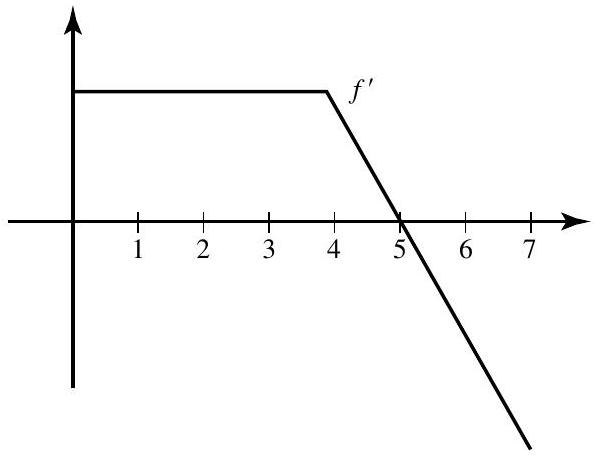
\includegraphics[width=0.40\linewidth]{calculus/images/7914d111-1a3f-478e-8520-371cc22a7467-08_458_597_389_695.jpg}
\end{center}
\end{EnvFullwidth}
\question\label{calc04:fggraph-first}
From the graph it follows that
\begin{choices}
  \choice $f$ is discontinuous at $x=4$
  \choice $f$ is decreasing for $4<x<7$
  \choice $f$ is constant for $0<x<4$
  \choice $f$ has a local maximum at $x=0$
  \CorrectChoice $f$ has a local minimum at $x=7$
\end{choices}
\begin{solution}
Since $f^{\prime}<0$ on $5 \leqslant x<7$, the function decreases as it approaches the right endpoint.
\end{solution}

\question
Which statement best describes $f$ at $x=5$ ?
\begin{choices}
  \choice $f$ has a root.
  \CorrectChoice $f$ has a maximum.
  \choice $f$ has a minimum.
  \choice The graph of $f$ has a point of inflection.
  \choice none of these
\end{choices}
\begin{solution}
For $x<5, f^{\prime}>0$, so $f$ is increasing; for $x>5, f$ is decreasing.
\end{solution}

\question\label{calc04:fggraph-last}
For which interval is the graph of $f$ concave downward?
\begin{choices}
  \choice $(0,4)$
  \choice $(4,5)$
  \choice $(5,7)$
  \CorrectChoice $(4,7)$
  \choice none of these
\end{choices}
\begin{solution}
The graph of $f$ being concave downward implies that $f^{\prime \prime}<0$, which implies that $f^{\prime}$ is decreasing.
\end{solution}





\newpage




\begin{EnvFullwidth}
\textit{Use the graph shown for Questions~\ref{calc04:velgraph-first}--\ref{calc04:velgraph-last}. It shows the velocity of an object moving along a straight line during the time interval $0 \leqslant t \leqslant 5$.}
\begin{center}
  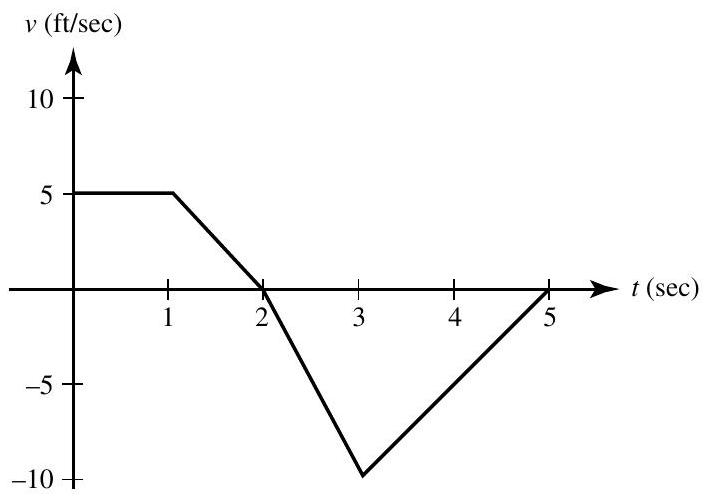
\includegraphics[width=0.60\linewidth]{calculus/images/7914d111-1a3f-478e-8520-371cc22a7467-08_502_711_1825_633.jpg}
\end{center}
\end{EnvFullwidth}
\question\label{calc04:velgraph-first}
The object attains its maximum speed when $t=$
\begin{choices}
  \choice $0$
  \choice $1$
  \choice $2$
  \CorrectChoice $3$
  \choice $5$
\end{choices}
\begin{solution}
Speed is the magnitude of velocity; at $t=3$, speed $=10 \mathrm{ft} / \mathrm{sec}$.
\end{solution}

\question
The speed of the object is increasing during the time interval
\begin{choices}
  \choice $(0,1)$
  \choice $(1,2)$
  \choice $(0,2)$
  \CorrectChoice $(2,3)$
  \choice $(3,5)$
\end{choices}
\begin{solution}
Speed increases from 0 at $t=2$ to 10 at $t=3$; it is constant or decreasing elsewhere.
\end{solution}





\newpage




\question
The acceleration of the object is positive during the time interval
\begin{choices}
  \choice $(0,1)$
  \choice $(1,2)$
  \choice $(0,2)$
  \choice $(2,3)$
  \CorrectChoice $(3,5)$
\end{choices}
\begin{solution}
Acceleration is positive when the velocity increases.
\end{solution}

\question
How many times on $0<t<5$ is the object's acceleration undefined?
\begin{choices}
  \choice none
  \choice $1$
  \choice $2$
  \CorrectChoice $3$
  \choice more than $3$
\end{choices}
\begin{solution}
Acceleration is undefined when velocity is not differentiable. Here that occurs at $t=1,2,3$.
\end{solution}

\question
During $2<t<3$ the object's acceleration (in $\mathrm{ft} / \mathrm{sec}^{2}$ ) is
\begin{choices}
  \CorrectChoice $-10$
  \choice $-5$
  \choice $0$
  \choice $5$
  \choice $10$
\end{choices}
\begin{solution}
Acceleration is the derivative of velocity. Since the velocity is linear, its derivative is its slope.
\end{solution}

\question
The object is furthest to the right when $t=$
\begin{choices}
  \choice $0$
  \choice $1$
  \CorrectChoice $2$
  \choice $3$
  \choice $5$
\end{choices}
\begin{solution}
Positive velocity implies motion to the right $(t<2)$; negative velocity $(t>2)$ implies motion to the left.
\end{solution}





\newpage




\question\label{calc04:velgraph-last}
The object's average acceleration (in $\mathrm{ft} / \mathrm{sec}^{2}$ ) for the interval $0 \leqslant t \leqslant 3$ is
\begin{choices}
  \choice $-15$
  \CorrectChoice $-5$
  \choice $-3$
  \choice $-1$
  \choice none of these
\end{choices}
\begin{solution}
The average rate of change of velocity is $\dfrac{v(3)-v(0)}{3-0}=\dfrac{-10-5}{-3} \mathrm{ft} / \mathrm{sec}^{2}$.
\end{solution}






\question
The line $y=3 x+k$ is tangent to the curve $y=x^{3}$ when $k$ is equal to
\begin{choices}
  \choice $1$ or $-1$
  \choice $0$
  \choice $3$ or $-3$
  \choice $4$ or $-4$
  \CorrectChoice $2$ or $-2$
\end{choices}
\begin{solution}
The slope of $y=x^{3}$ is $3 x^{2}$. It is equal to 3 when $x= \pm 1$. At $x=1$, the equation of the tangent is
\[
y-1=3(x-1) \quad \text { or } \quad y=3 x+2
\]
At $x=-1$, the equation is
\[
y+1=3(x+1) \quad \text { or } \quad y=3 x+2
\]
\end{solution}





\newpage




\question
The two tangents that can be drawn from the point $(3,5)$ to the parabola $y=x^{2}$ have slopes
\begin{choices}
  \choice $1$ and $5$
  \choice $0$ and $4$
  \CorrectChoice $2$ and $10$
  \choice $2$ and $-\dfrac{1}{2}$
  \choice $2$ and $4$
\end{choices}
\begin{solution}
Let the tangent to the parabola from $(3,5)$ meet the curve at $\left(x_{1}, y_{1}\right)$. Its equation is $y-5=2 x_{1}(x-3)$. Since the point ( $x_{1}, y_{1}$ ) is on both the tangent and the parabola, we solve simultaneously:
\[
y_{1}-5=2 x_{1}\left(x_{1}-3\right) \quad \text { and } \quad y_{1}=x_{1}^{2}
\]
The points of tangency are $(5,25)$ and $(1,1)$. The slopes, which equal $2 x_{1}$, are 10 and 2.
\end{solution}

\question
The table shows the velocity at various times of an object moving along a line. An estimate of its acceleration (in $\mathrm{ft} / \mathrm{sec}^{2}$ ) at $t=1$ is

\begin{center}
\begin{tabular}{l|r|r|r|r}
$t(\mathrm{sec})$ & 1.0 & 1.5 & 2.0 & 2.5 \\
\hline
$v(\mathrm{ft} / \mathrm{sec})$ & 12.2 & 13.0 & 13.4 & 13.7 \\
\end{tabular}
\end{center}
\begin{choices}
  \choice $0.8$
  \choice $1.0$
  \choice $1.2$
  \choice $1.4$
  \CorrectChoice $1.6$
\end{choices}
\begin{solution}
$a \simeq \dfrac{\Delta v}{\Delta t}=\dfrac{v(1.5)-v(1.0)}{0.5}=\dfrac{13.2-12.2}{0.5} \mathrm{ft} / \mathrm{sec}^{2}$.
\end{solution}





\newpage




\begin{EnvFullwidth}
\textit{For Questions~\ref{calc04:fsin-first}--\ref{calc04:fsin-last}, $f^{\prime}(x)=x \sin x-\cos x$ for $0<x<4$.}
\end{EnvFullwidth}

\question\label{calc04:fsin-first}
$f$ has a local maximum when $x$ is approximately
\begin{choices}
  \choice $0.9$
  \choice $1.2$
  \choice $2.3$
  \CorrectChoice $3.4$
  \choice $3.7$
\end{choices}
\begin{solution}
The graph of $f^{\prime}(x)=x \sin x-\cos x$ is drawn here in the window $[0,4] \times[-3,3]$ :
\begin{center}
  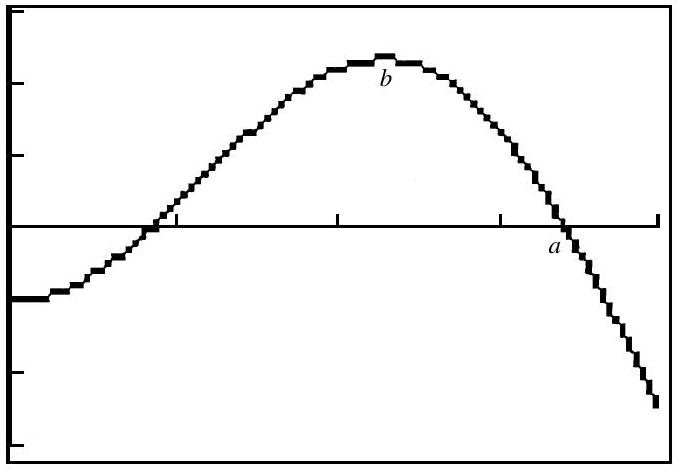
\includegraphics[width=0.40\linewidth]{calculus/images/7914d111-1a3f-478e-8520-371cc22a7467-21_472_680_1298_1011.jpg}
\end{center}
A local maximum exists where $f^{\prime}$ changes from positive to negative; use your calculator to approximate $a$.
\end{solution}

\question\label{calc04:fsin-last}
The graph of $f$ has a point of inflection when $x$ is approximately
\begin{choices}
  \choice $0.9$
  \choice $1.2$
  \CorrectChoice $2.3$
  \choice $3.4$
  \choice $3.7$
\end{choices}
\begin{solution}
$f^{\prime \prime}$ changes sign when $f^{\prime}$ changes from increasing to decreasing (or vice versa). Again, use your calculator to approximate the $x$-coordinate at $b$.
\end{solution}




\newpage





\begin{EnvFullwidth}
\textit{In Questions~\ref{calc04:plane-first}--\ref{calc04:plane-last}, the motion of a particle in a plane is given by the pair of equations $x=2 t$ and $y=4 t-t^{2}$.}
\end{EnvFullwidth}

\question\label{calc04:plane-first}
The particle moves along
\begin{choices}
  \choice an ellipse
  \choice a circle
  \choice a hyperbola
  \choice a line
  \CorrectChoice a parabola
\end{choices}
\begin{solution}
(E) Eliminating $t$ yields the equation $y=-\dfrac{1}{4} x^{2}+2 x$.
\end{solution}

\question
The speed of the particle at any time $t$ is
\begin{choices}
  \choice $\sqrt{6-2 t}$
  \CorrectChoice $2 \sqrt{t^{2}-4 t+5}$
  \choice $2 \sqrt{t^{2}-2 t+5}$
  \choice $\sqrt{8}(|t-2|)$
  \choice $2(|3-t|)$
\end{choices}
\begin{solution}
(B) $\quad|\mathbf{v}|=\sqrt{\left(\dfrac{d x}{d t}\right)^{2}+\left(\dfrac{d y}{d t}\right)^{2}}=\sqrt{2^{2}+(4-2 t)^{2}}$.
\end{solution}

\question
The minimum speed of the particle is
\begin{choices}
  \CorrectChoice $2$
  \choice $2 \sqrt{2}$
  \choice $0$
  \choice $1$
  \choice $4$
\end{choices}
\begin{solution}
(A) Since $|\mathbf{v}|=2 \sqrt{t^{2}-4 t+5}, \dfrac{d|\mathbf{v}|}{d t}=\dfrac{2 t-4}{\sqrt{t^{2}-4 t+5}}=0$ if $t=2$. We note that, as $t$ increases through 2 , the signs of $|\mathbf{v}|^{\prime}$ are $-, 0,+$, assuring a minimum of $|\mathbf{v}|$ at $t=2$. Evaluate $|\mathbf{v}|$ at $t=2$.
\end{solution}





\newpage




\question\label{calc04:plane-last}
The acceleration of the particle
\begin{choices}
  \choice depends on $t$
  \choice is always directed upward
  \CorrectChoice is constant both in magnitude and in direction
  \choice never exceeds $1$ in magnitude
  \choice is none of these
\end{choices}
\begin{solution}
(C) The direction of $\mathbf{a}$ is $\tan ^{-1} \dfrac{\dfrac{d^{2} y}{d t^{2}}}{\dfrac{d^{2} x}{d t^{2}}}$. Since $\dfrac{d^{2} x}{d t^{2}}=0$ and $\dfrac{d^{2} y}{d t^{2}}=-2$, the acceleration is always directed downward. Its magnitude, $\sqrt{0^{2}+(-2)^{2}}$, is 2 for all $t$.
\end{solution}

\question
If a particle moves along a curve with constant speed, then
\begin{choices}
  \choice the magnitude of its acceleration must equal zero
  \choice the direction of acceleration must be constant
  \choice the curve along which the particle moves must be a straight line
  \CorrectChoice its velocity and acceleration vectors must be perpendicular
  \choice the curve along which the particle moves must be a circle
\end{choices}
\begin{solution}
(D) Using the notations $v_{x}, v_{y}, a_{x}$, and $a_{y}$, we are given that $|\mathbf{v}|=\sqrt{v_{x}^{2}+v_{y}^{2}}=k$, where $k$ is a constant. Then
\[
\dfrac{d|\mathbf{v}|}{d t}=\dfrac{v_{x} a_{x}+v_{y} a_{y}}{|\mathbf{v}|}=0 \quad \text { or } \quad \dfrac{v_{x}}{v_{y}}=-\dfrac{a_{y}}{a_{x}} .
\]
\end{solution}

\question
A particle is moving on the curve of $y=2 x-\ln x$ so that $\dfrac{d x}{d t}=-2$ at all times $t$. At the point $(1,2), \dfrac{d y}{d t}$ is
\begin{choices}
  \choice $4$
  \choice $2$
  \choice $-4$
  \choice $1$
  \CorrectChoice $-2$
\end{choices}
\begin{solution}
$\dfrac{d y}{d t}=\left(2-\dfrac{1}{x}\right) \dfrac{d x}{d t}=\left(2-\dfrac{1}{x}\right)(-2)$.
\end{solution}





\newpage




\begin{EnvFullwidth}
\textit{Use the graph of $f^{\prime}$ on $[0,5]$, shown below, for Questions~\ref{calc04:fprime-first}--\ref{calc04:fprime-last}.}
\begin{center}
  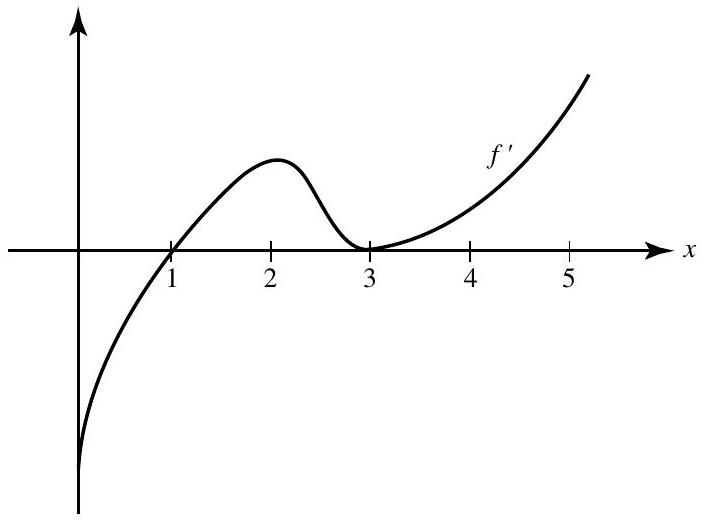
\includegraphics[width=0.60\linewidth]{calculus/images/7914d111-1a3f-478e-8520-371cc22a7467-11_523_706_431_1013.jpg}
\end{center}
\end{EnvFullwidth}

\question\label{calc04:fprime-first}
$f$ has a local minimum at $x=$
\begin{choices}
  \choice $0$
  \CorrectChoice $1$
  \choice $2$
  \choice $3$
  \choice $5$
\end{choices}
\begin{solution}
A local minimum exists where $f$ changes from decreasing $\left(f^{\prime}<0\right)$ to increasing $\left(f^{\prime}>0\right)$. Note that $f$ has local maxima at both endpoints, $x=0$ and $x=5$.
\end{solution}

\question\label{calc04:fprime-last}
The graph of $f$ has a point of inflection at $x=$
\begin{choices}
  \choice $1$ only
  \choice $2$ only
  \choice $3$ only
  \CorrectChoice $2$ and $3$ only
  \choice none of these
\end{choices}
\begin{solution}
See Question~\ref{calc04:fsin-last}.
\end{solution}





\newpage




\question
It follows from the graph of $f^{\prime}$, shown at the right, that
\begin{center}
  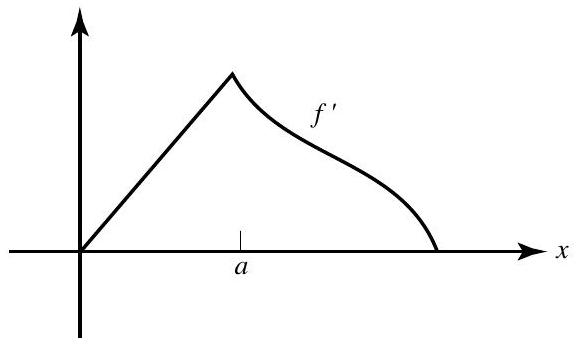
\includegraphics[width=0.60\linewidth]{calculus/images/7914d111-1a3f-478e-8520-371cc22a7467-11_347_577_1382_1458.jpg}
\end{center}
\begin{choices}
  \choice $f$ is not continuous at $x=a$
  \choice $f$ is continuous but not differentiable at $x=a$
  \choice $f$ has a relative maximum at $x=a$
  \CorrectChoice The graph of $f$ has a point of inflection at $x=a$
  \choice none of these
\end{choices}
\begin{solution}
$f^{\prime}$ changes from increasing $\left(f^{\prime \prime}>0\right)$ to decreasing $\left(f^{\prime \prime}<0\right)$. Note that $f$ is differentiable at $a$ (because $f^{\prime}(a)$ exists) and therefore continuous at $a$.
\end{solution}

\question
A vertical circular cylinder has radius $r \mathrm{ft}$ and height $h \mathrm{ft}$. If the height and radius both increase at the constant rate of $2 \mathrm{ft} / \mathrm{sec}$, then the rate, in square feet per second, at which the lateral surface area increases is
\begin{choices}
  \choice $4 \pi r$
  \choice $2 \pi(r+h)$
  \CorrectChoice $4 \pi(r+h)$
  \choice $4 \pi r h$
  \choice $4 \pi h$
\end{choices}
\begin{solution}
We know that $\dfrac{d h}{d t}=\dfrac{d r}{d t}=2$. Since $S=2 \pi r h$,
\[
\dfrac{d S}{d t}=2 \pi\left(r \dfrac{d h}{d t}+h \dfrac{d r}{d t}\right)
\]
\end{solution}





\newpage




\question
A tangent drawn to the parabola $y=4-x^{2}$ at the point ( 1,3 ) forms a right triangle with the coordinate axes. The area of the triangle is
\begin{choices}
  \choice $\dfrac{5}{4}$
  \choice $\dfrac{5}{2}$
  \choice $\dfrac{25}{2}$
  \choice $1$
  \CorrectChoice $\dfrac{25}{4}$
\end{choices}
\begin{solution}
The equation of the tangent is $y=-2 x+5$. Its intercepts are $\dfrac{5}{2}$ and 5 .
\end{solution}

\question\label{calc04:cars}
Two cars are traveling along perpendicular roads, car $A$ at 40 mph , car $B$ at 60 mph . At noon, when car $A$ reaches the intersection, car $B$ is 90 mi away, and moving toward it. At 1 p.m. the rate, in miles per hour, at which the distance between the cars is changing is
\begin{choices}
  \choice $-40$
  \choice $68$
  \choice $4$
  \CorrectChoice $-4$
  \choice $40$
\end{choices}
\begin{solution}
See the figure. At noon, $\operatorname{car} A$ is at $O, \operatorname{car} B$ at $N$; the cars are shown $t$ hours after noon. We know that $\dfrac{d x}{d t}=-60$ and that $\dfrac{d y}{d t}=40$. Using $s^{2}=x^{2}+y^{2}$, we get
\[
\dfrac{d s}{d t}=\dfrac{x \dfrac{d x}{d t}+y \dfrac{d y}{d t}}{s}=\dfrac{-60 x+40 y}{s} .
\]
\begin{center}
  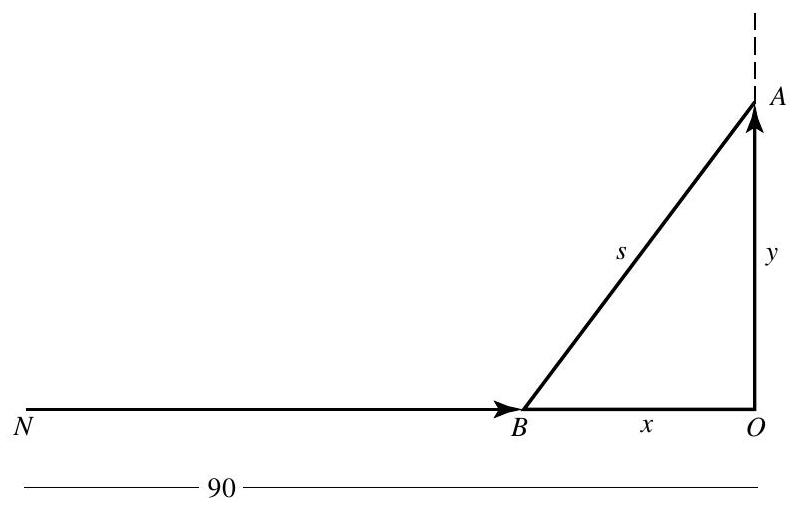
\includegraphics[width=0.40\linewidth]{calculus/images/7914d111-1a3f-478e-8520-371cc22a7467-22_511_799_2006_586.jpg}
\end{center}
At 1 P.M., $x=30, y=40$, and $s=50$.
\end{solution}





\newpage




\question
For Question~\ref{calc04:cars}, if $t$ is the number of hours of travel after noon, then the cars are closest together when $t$ is
\begin{choices}
  \choice $0$
  \CorrectChoice $\dfrac{27}{26}$
  \choice $\dfrac{9}{5}$
  \choice $\dfrac{3}{2}$
  \choice $\dfrac{14}{13}$
\end{choices}
\begin{solution}
$\dfrac{d s}{d t}$ (from Question~\ref{calc04:cars}) is zero when $y=\dfrac{3}{2} x$. Note that $x=90-60 t$ and $y=40 t$.
\end{solution}





\newpage




\begin{EnvFullwidth}
\textit{The graph for Questions~\ref{calc04:vel2-first}--\ref{calc04:vel2-last} shows the velocity of an object moving along a straight line during the time interval $0 \leqslant t \leqslant 12$.}
\begin{center}
  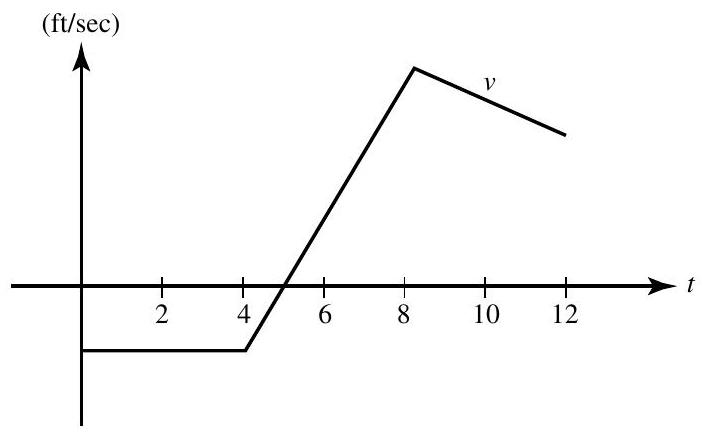
\includegraphics[width=0.7\linewidth]{calculus/images/7914d111-1a3f-478e-8520-371cc22a7467-12_434_706_691_635.jpg}
\end{center}
\end{EnvFullwidth}

\question\label{calc04:vel2-first}
For what $t$ does this object attain its maximum acceleration?
\begin{choices}
  \choice $0<t<4$
  \CorrectChoice $4<t<8$
  \choice $t=5$
  \choice $t=8$
  \choice $t=12$
\end{choices}
\begin{solution}
(B) Maximum acceleration occurs when the derivative (slope) of velocity is greatest.
\end{solution}

\question\label{calc04:vel2-last}
The object reverses direction at $t=$
\begin{choices}
  \choice $4$ only
  \CorrectChoice $5$ only
  \choice $8$ only
  \choice $5$ and $8$
  \choice none of these
\end{choices}
\begin{solution}
(B) The object changes direction only when velocity changes sign. Velocity changes sign from negative to positive at $t=5$.
\end{solution}





\newpage




\question
The graph of $f^{\prime}$ is shown below. If we know that $f(2)=10$, then the local linearization of $f$ at $x=2$ is $f(x) \simeq$
\begin{center}
  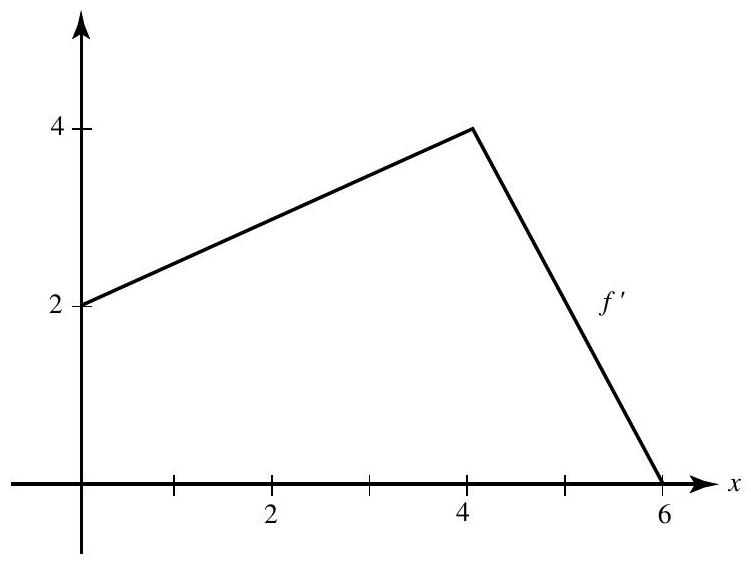
\includegraphics[width=0.60\linewidth]{calculus/images/7914d111-1a3f-478e-8520-371cc22a7467-12_565_751_1892_630.jpg}
\end{center}
\begin{choices}
  \choice $\dfrac{x}{2}+2$
  \choice $\dfrac{x}{2}+9$
  \choice $3 x-3$
  \CorrectChoice $3 x+4$
  \choice $10 x-17$
\end{choices}
\begin{solution}
(D) From the graph, $f^{\prime}(2)=3$, and we are told the line passes through $(2,10)$. We therefore have $f(x) \simeq 10+3(x-2)=3 x+4$.
\end{solution}





\newpage




\question
Given $f^{\prime}$ as graphed, which could be the graph of $f$ ?
\begin{center}
  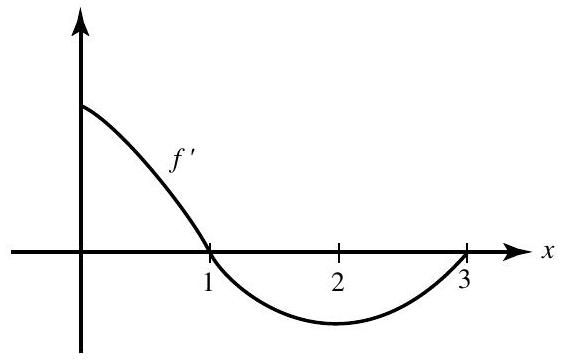
\includegraphics[width=0.7\linewidth]{calculus/images/7914d111-1a3f-478e-8520-371cc22a7467-13_362_563_429_1050.jpg}
\end{center}
\begin{oneparchoices}
\choice
\begin{minipage}[t]{0.28\linewidth}
  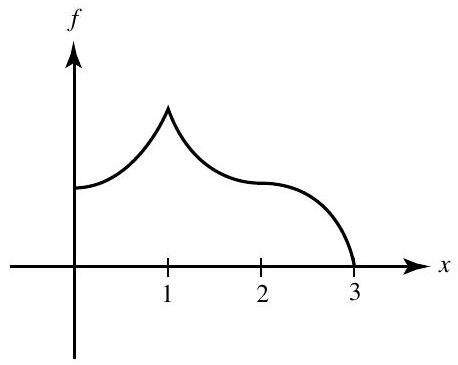
\includegraphics[width=\linewidth]{calculus/images/7914d111-1a3f-478e-8520-371cc22a7467-13_365_458_941_719.jpg}
\end{minipage}
\choice
\begin{minipage}[t]{0.28\linewidth}
  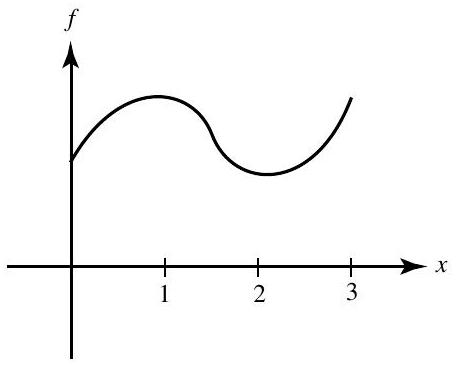
\includegraphics[width=\linewidth]{calculus/images/7914d111-1a3f-478e-8520-371cc22a7467-13_365_458_941_1396.jpg}
\end{minipage}
\CorrectChoice
\begin{minipage}[t]{0.28\linewidth}
  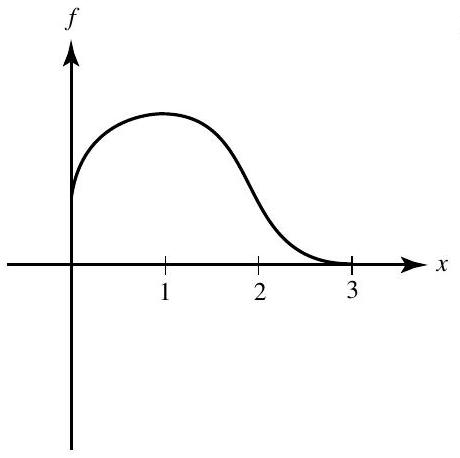
\includegraphics[width=\linewidth]{calculus/images/7914d111-1a3f-478e-8520-371cc22a7467-13_458_460_1377_533.jpg}
\end{minipage}
\par\vspace{10pt}\noindent
\choice
\begin{minipage}[t]{0.28\linewidth}
  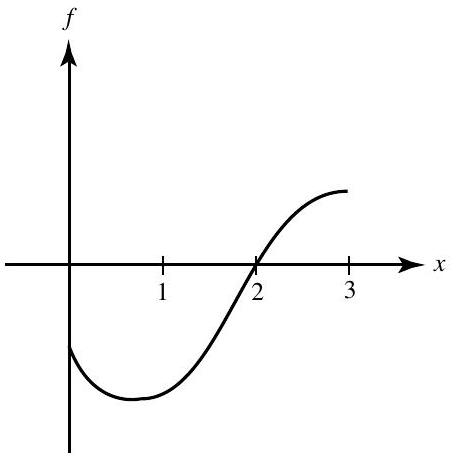
\includegraphics[width=\linewidth]{calculus/images/7914d111-1a3f-478e-8520-371cc22a7467-13_463_458_1377_1053.jpg}
\end{minipage}
\choice
\begin{minipage}[t]{0.28\linewidth}
  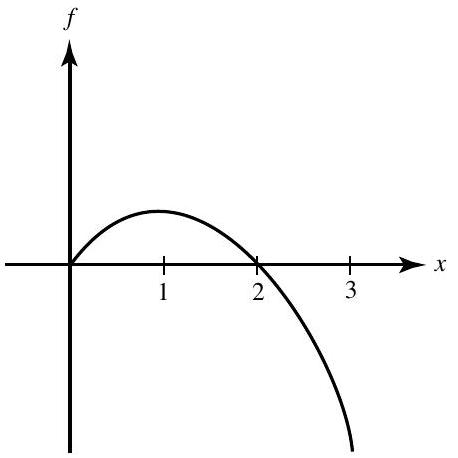
\includegraphics[width=\linewidth]{calculus/images/7914d111-1a3f-478e-8520-371cc22a7467-13_458_458_1377_1577.jpg}
\end{minipage}
\end{oneparchoices}
\begin{solution}
At $x=1$ and $3, f^{\prime}(x)=0$; therefore $f$ has horizontal tangents.

For $x<1, f^{\prime}>0$; therefore $f$ is increasing.

For $x>1, f^{\prime}<0$, so $f$ is decreasing.

For $x<2, f^{\prime}$ is decreasing, so $f^{\prime \prime}<0$ and the graph of $f$ is concave downward.

For $x>2, f^{\prime}$ is increasing, so $f^{\prime \prime}>0$ and the graph of $f$ is concave upward.
\end{solution}





\newpage




\begin{EnvFullwidth}
\textit{Use the following graph for Questions~\ref{calc04:labeled-first}--\ref{calc04:labeled-last}.}
\begin{center}
  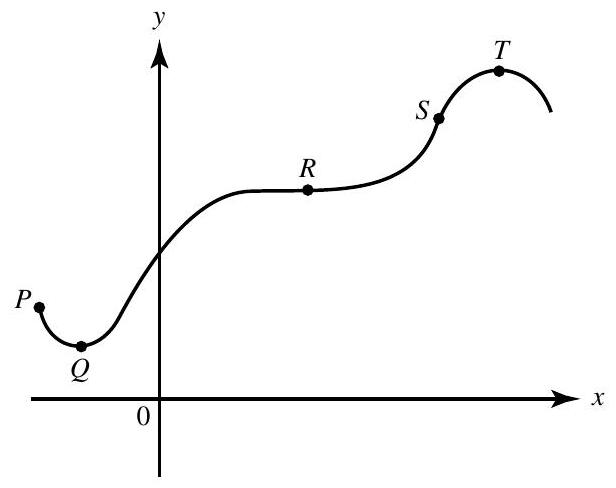
\includegraphics[width=0.60\linewidth]{calculus/images/7914d111-1a3f-478e-8520-371cc22a7467-14_488_616_373_679.jpg}
\end{center}
\end{EnvFullwidth}

\question\label{calc04:labeled-first}
At which labeled point do both $\dfrac{d y}{d x}$ and $\dfrac{d^{2} y}{d x^{2}}$ equal zero?
\begin{choices}
  \choice $P$
  \choice $Q$
  \CorrectChoice $R$
  \choice $S$
  \choice $T$
\end{choices}
\begin{solution}
(C) Note that $\dfrac{d y}{d x}=0$ at $Q, R$, and $T$. At $Q, \dfrac{d^{2} y}{d x^{2}}>0$; at $T, \dfrac{d^{2} y}{d x^{2}}<0$.
\end{solution}

\question
At which labeled point is $\dfrac{d y}{d x}$ positive and $\dfrac{d^{2} y}{d x^{2}}$ equal to zero?
\begin{choices}
  \choice $P$
  \choice $Q$
  \choice $R$
  \CorrectChoice $S$
  \choice $T$
\end{choices}
\begin{solution}
(D) Only at $S$ does the graph both rise and change concavity.
\end{solution}





\newpage




\question\label{calc04:labeled-last}
At which labeled point is $\dfrac{d y}{d x}$ equal to zero and $\dfrac{d^{2} y}{d x^{2}}$ negative?
\begin{choices}
  \choice $P$
  \choice $Q$
  \choice $R$
  \choice $S$
  \CorrectChoice $T$
\end{choices}
\begin{solution}
Only at $T$ is the tangent horizontal and the curve concave down.
\end{solution}

\question
If $f(6)=30$ and $f^{\prime}(x)=\dfrac{x^{2}}{x+3}$, estimate $f(6.02)$ using the line tangent to $f$ at $x=6$.
\begin{choices}
  \choice $29.92$
  \choice $30.02$
  \CorrectChoice $30.08$
  \choice $34.00$
  \choice none of these
\end{choices}
\begin{solution}
(C) Since $f^{\prime}(6)=4$, the equation of the tangent at $(6,30)$ is $y-30=4(x-6)$. Therefore $f(x) \simeq 4 x+6$ and $f(6.02) \simeq 30.08$.
\end{solution}

\question
The tangent line approximation for $f(x)=\sqrt{x^{2}+16}$ near $x=-3$ is
\begin{choices}
  \choice $5-\dfrac{3}{5}(x-3)$
  \choice $5+\dfrac{3}{5}(x-3)$
  \CorrectChoice $5-\dfrac{3}{5}(x+3)$
  \choice $3-\dfrac{5}{3}(x-3)$
  \choice $3+\dfrac{3}{5}(x+3)$
\end{choices}
\begin{solution}
(C) $\sqrt{x^{2}+16} \simeq \sqrt{9+16}+\dfrac{(-3)}{\sqrt{(-3)^{2}+16}}(x+3)=5-\dfrac{3}{5}(x+3)$
\end{solution}